%%%%%%%%%%%%%%%%%%%%%%%%%%%%%%%%%%%%%%%%%

%%%%%%%%%%%%%%%%%%%%%%%%%%%%%%%%%%%%%%%%%

\documentclass[12pt]{article} % Default font size is 12pt, it can be changed here

\usepackage{geometry} % Required to change the page size to A4
\geometry{a4paper} % Set the page size to be A4 as opposed to the default US Letter

\usepackage{graphicx} % Required for including pictures

\usepackage{float} % Allows putting an [H] in \begin{figure} to specify the exact location of the figure
\usepackage{wrapfig} % Allows in-line images such as the example fish picture
\usepackage{caption}

\usepackage{lipsum} % Used for inserting dummy 'Lorem ipsum' text into the template

\linespread{1.2} % Line spacing

%\setlength\parindent{0pt} % Uncomment to remove all indentation from paragraphs

\graphicspath{{./Pictures/}} % Specifies the directory where pictures are stored

\begin{document}

%----------------------------------------------------------------------------------------
%	TITLE PAGE
%----------------------------------------------------------------------------------------

\begin{titlepage}

\newcommand{\HRule}{\rule{\linewidth}{0.5mm}} % Defines a new command for the horizontal lines, change thickness here

\center % Center everything on the page

\textsc{\LARGE Carnegie Mellon University}\\[1.5cm] % Name of your university/college
\textsc{\Large Master of Science in Music and Technology}\\[0.5cm] % Major heading such as course name

\HRule \\[0.4cm]
{\large \bfseries A Proposal for a Music Player \\ for the Human Computer Music Performance Project}\\[0.4cm] % Title of your document
\HRule \\[1.5cm]

\begin{minipage}{0.4\textwidth}
\begin{flushleft} \large
\emph{Author:}\\
Dalong \textsc{Cheng} % Your name
\end{flushleft}
\end{minipage}
~
\begin{minipage}{0.4\textwidth}
\begin{flushright} \large
\emph{Supervisor:} \\
Roger \textsc{Dannenberg} \\ % Supervisor's Name
Richard \textsc{Stern} \\
Richard \textsc{Randall}
\end{flushright}
\end{minipage}\\[4cm]

{\large \today}\\[3cm] % Date, change the \today to a set date if you want to be precise

%\includegraphics{Logo}\\[1cm] % Include a department/university logo - this will require the graphicx package

\vfill % Fill the rest of the page with whitespace



%----------------------------------------------------------------------------------------
%	TABLE OF CONTENTS
%----------------------------------------------------------------------------------------
\end{titlepage}

\tableofcontents % Include a table of contents
\setcounter{page}{2}
\pagenumbering{roman}

\newpage % Begins the essay on a new page instead of on the same page as the table of contents 

%----------------------------------------------------------------------------------------
%	INTRODUCTION
%----------------------------------------------------------------------------------------

\pagestyle{headings}
\setcounter{page}{1}
\pagenumbering{arabic}

%Example citation \cite{Figueredo:2009dg}
\section{Introduction} % Major section

The goal of the Human Computer Music Performance (HCMP) \cite{Dawen:2011} project is to create an autonomous 
``artificial performer'' with the ability of a human-level musical performance. 
An important component of the HCMP project is to develop a player component, which can flexibly  
adjust and respond to changes in a music signal. Figure 1 illustrates the role of the Player in the HCMP
project. The Player will receive control messages from the conductor and scheduler during the performance. 
In my master's project, I will design, implement and extend the HCMP midi player for the HCMP project. 

\begin{figure}[H] % Example image
\center{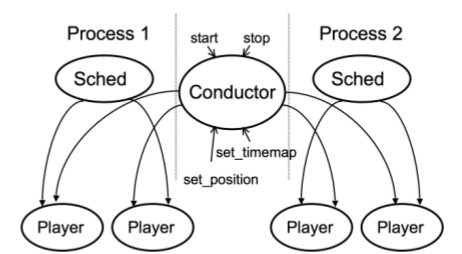
\includegraphics[width=0.5\linewidth]{1.png}}
\caption{Architecture of HCMP}
\label{fig:speciation}
\end{figure}
%------------------------------------------------

\subsection{Software Architecture} % Sub-section
In this project, I will use a classic client and server model for the overall architecture. 
During the performance, the Player will act as the server for the conductor component, which is constantly 
receiving control messages and responding accordingly. 

Internally, the Player will have two threads, with one thread for
GUI interactive control (control thread) and the other thread for performing music data (performer thread). 
The two threads will communicate with each other through a shared message queue, we can assume the message 
queue is large enough to avoid blocks for both caller and callee threads. The performaner thread
will handle time critical operations, and there will be a timer setup before this thread is created. The goal of the timer is to 
wake up the performer thread periodically. Everytime the performer thread's timer callback function is invoked, 
it will check the message queue and process any command from the control thread. 
Figure 2 illustrates the overall structure of the Player.

\begin{figure}[H] % Example image
\center{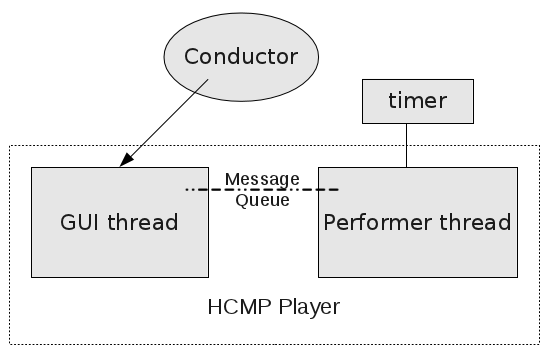
\includegraphics[width=0.5\linewidth]{2.png}}
\caption{Architecture of the HCMP Midi Player}
\label{fig:speciation}
\end{figure}

\subsection{HCMP Midi Player Mode} % Sub-section
The Player will have two modes, stand-alone
mode and connection mode. The user is able to switch between the two. In stand-alone mode, 
the Player is similar to a standard midi player, which can play midi  
files and set various playback parameters. All user operations will go through the GUI to control. 
In connection mode the Player will use a predefined protocol to communicate with the conductor and all the 
control messages will be received from a remote conductor. In connection mode the GUI will use another 
set of function to map the user operation and some functions of the Player will be controlled by the 
remote conductor. The control thread 
of the Player will act as a ``proxy'': on one side, 
it will receive the message from the conductor, on the other side, it will issue a new control message
to the performer thread.

%----------------------------------------------------------------------------------------
%	MAJOR SECTION 1
%----------------------------------------------------------------------------------------

\section{General Design} % Major section

In this part, I describe the design idea behind some of the features of the Player. 

\subsection{HCMP Midi Player GUI Design} % Sub-section

\subsubsection{Midi Keyboard and Data Display} % Sub-sub-section
The Player will contain a virtual keyboard and midi data window. The 
virtual keyboard will have parameters like channel, tempo, etc for the user to set. 
It will also be integrated with a midi data window to improve the data visualization
effect. After loading a midi file, the midi data window will map each midi note to a key on the midi keyboard. 
When playing the midi file, the keyboard will highlight each midi note, the midi data window
will scroll to the current message position.

\begin{figure}[H] % Example image
\center{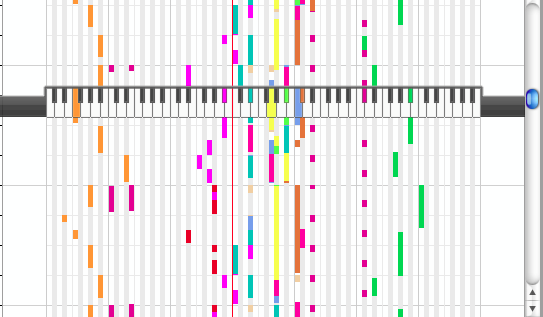
\includegraphics[width=0.5\linewidth]{3.png}}
\caption{Midi data display integrated with vitural keyboard}
\label{fig:speciation}
\end{figure}

\subsection{HCMP Midi Player Library}
The Player will also generate a configration file to manage and 
save configurations set by the user. The Player has a simple to  
use midi library to manage recently played midi information. Figure 4 is an ideal interface
for the midi library.
\begin{figure}[H] % Example image
\center{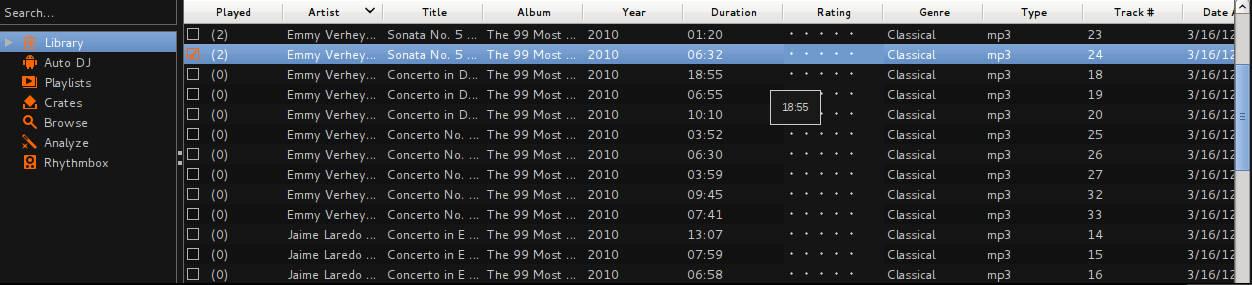
\includegraphics[width=0.8\linewidth]{4.png}}
\caption{HCMP Midi player library}
\label{fig:speciation}
\end{figure}

\subsection{HCMP Midi Player API}
In this section, I list some of the core APIs of the HCMP Midi Player. These APIs will be  
called by the GUI of the HCMP Player.\\
Music play related APIs
\begin{itemize}
  \item \texttt{play - play midi message}  
  \item \texttt{reset - reset all the player's settings to default value}  
  \item \texttt{pause - store current play information}
  \item \texttt{set\_position - set play position to the given parameter}
\end{itemize}
Player setting related APIs
\begin{itemize}
  \item \texttt{set\_track - set track for the player to play}  
  \item \texttt{set\_tempo - set tempo information }  
  \item \texttt{set\_channel - set channel information}
  \item \texttt{set\_device - set which midi device to send messages to}
\end{itemize}
Connection mode related APIs, which is inherited from Zero MQ \cite{zeromq}
\begin{itemize}
  \item \texttt{play\_all - indicate conductor to play}  
  \item \texttt{stop\_all - indicate conductor to stop}  
  \item \texttt{ready - tell the conductor that the player is ready}
  \item \texttt{position - indicate conductor to set to given position}
\end{itemize}

\section{Implementation}
The project will use Serpent \cite{Serpent} to develop most of the parts, because it has many 
convenient built in functions for midi messages. For the GUI part, I will use 
wxWidgets \cite{wxWidget}. The first priority of master's project is to deliver
a solid and robust midi player. I will design unit test code for each of the functional components 
during development.

\subsection{Performer Thread}
The performer thread will only receive control messages from the control thread. 
It will immediately process the message upon receiving it. This thread will be periodically invoked by 
an external timer, provided by Serpent, and process midi message sent from the control thread. 
Processing the message is not a time consuming job so the overall overhead of waking up 
thread will be trivial. Most of work of the performer thread is to maintain a queue of pending
midi message and send them at correct time.

\section{Future Work}
This proposal will provide a base for some future work. The Player will  
be integrated into the HCMP project. Two other features can be
added to extend the Player's function. There is a music score display component for the HCMP project. The Player can 
be used as a default player for music display component. Display with the addition of a midi 
score follower, the music display could be synchronized to a live keyboard performance and the Player could play 
an accompaniment part and the user can 
read the score from the Player's virtual keyboard. Dawen Liang's previous work 
\cite{Dawen:ISMIR2011}on music database provide user a convenient way to record, organize
and retrieve audio information from various sources. The Player can further integrate 
this feature to provide a powerful audio library management tool. 

%----------------------------------------------------------------------------------------
%	CONCLUSION
%----------------------------------------------------------------------------------------

%----------------------------------------------------------------------------------------
%	BIBLIOGRAPHY
%----------------------------------------------------------------------------------------

\begin{thebibliography}{99} % Bibliography - this is intentionally simple in this template

\bibitem{Dawen:2011}
Framework for Coordination and Synchronization of Media, D.Liang, G.Xia and R.Dannenberg, NIME 2011.

\bibitem{zeromq}
http://sourceforge.net/p/livedisp/wiki/HCMP%20messaging%20protocol/

\bibitem{Serpent}
http://www.cs.cmu.edu/~music/aura/serpent-info.htm

\bibitem{wxWidget}
http://www.wxwidget.org

\bibitem{Dawen:ISMIR2011}
Segmentation, Clustering, and Display in a Personal Music Database for Musicians,
G.Xia, D.Liang, R.Dannenberg, ISMIR 2011.

\end{thebibliography}

%----------------------------------------------------------------------------------------

\end{document}
